\documentclass[a4paper,12pt]{article}
\usepackage[T2A]{fontenc}
\usepackage[utf8]{inputenc}
\usepackage[russian]{babel}
\usepackage{graphicx}
\usepackage{float}
\usepackage{subcaption}
\usepackage{amsmath, amssymb}
\usepackage{geometry}
\geometry{top=2cm, bottom=2cm, left=3cm, right=1.5cm}

\begin{document}

\thispagestyle{empty}
\begin{center}
    \large
    Министерство науки и высшего образования Российской Федерации\\
    Федеральное государственное автономное образовательное учреждение\\
    высшего образования\\
    «Национальный исследовательский университет ИТМО»\\
    \vspace{5cm}
    \textbf{Отчёт по исследовательской работе № 1}\\
    \textbf{По предмету: Математический анализ и основы вычислений}\\
    \vspace{6cm}
    \begin{flushright}
        Выполнил работу:\\ Тиганов Вадим Игоревич\\
        \vspace{1cm}
        Академическая группа: \\ J3112\\
        \vspace{1cm}
        Вариант: \\18
    \end{flushright}
    \vspace{1cm}
    \vspace{3cm}
    \begin{center}
        Санкт-Петербург, 2025\\
    \end{center}
\end{center}

\newpage


\section{Ход работы}

\subsection{Задание 1}

Рассмотрим функцию
\[
f(x) = \frac{x^2 + 1}{x - 1}.
\]
Исследовать на равномерную непрерывность на множествах\\
\emph{(a)} \( X = [3, +\infty) \) \\
\emph{(b)} \( X = (1, 3) \)\\

\begin{figure}[h]
    \centering
    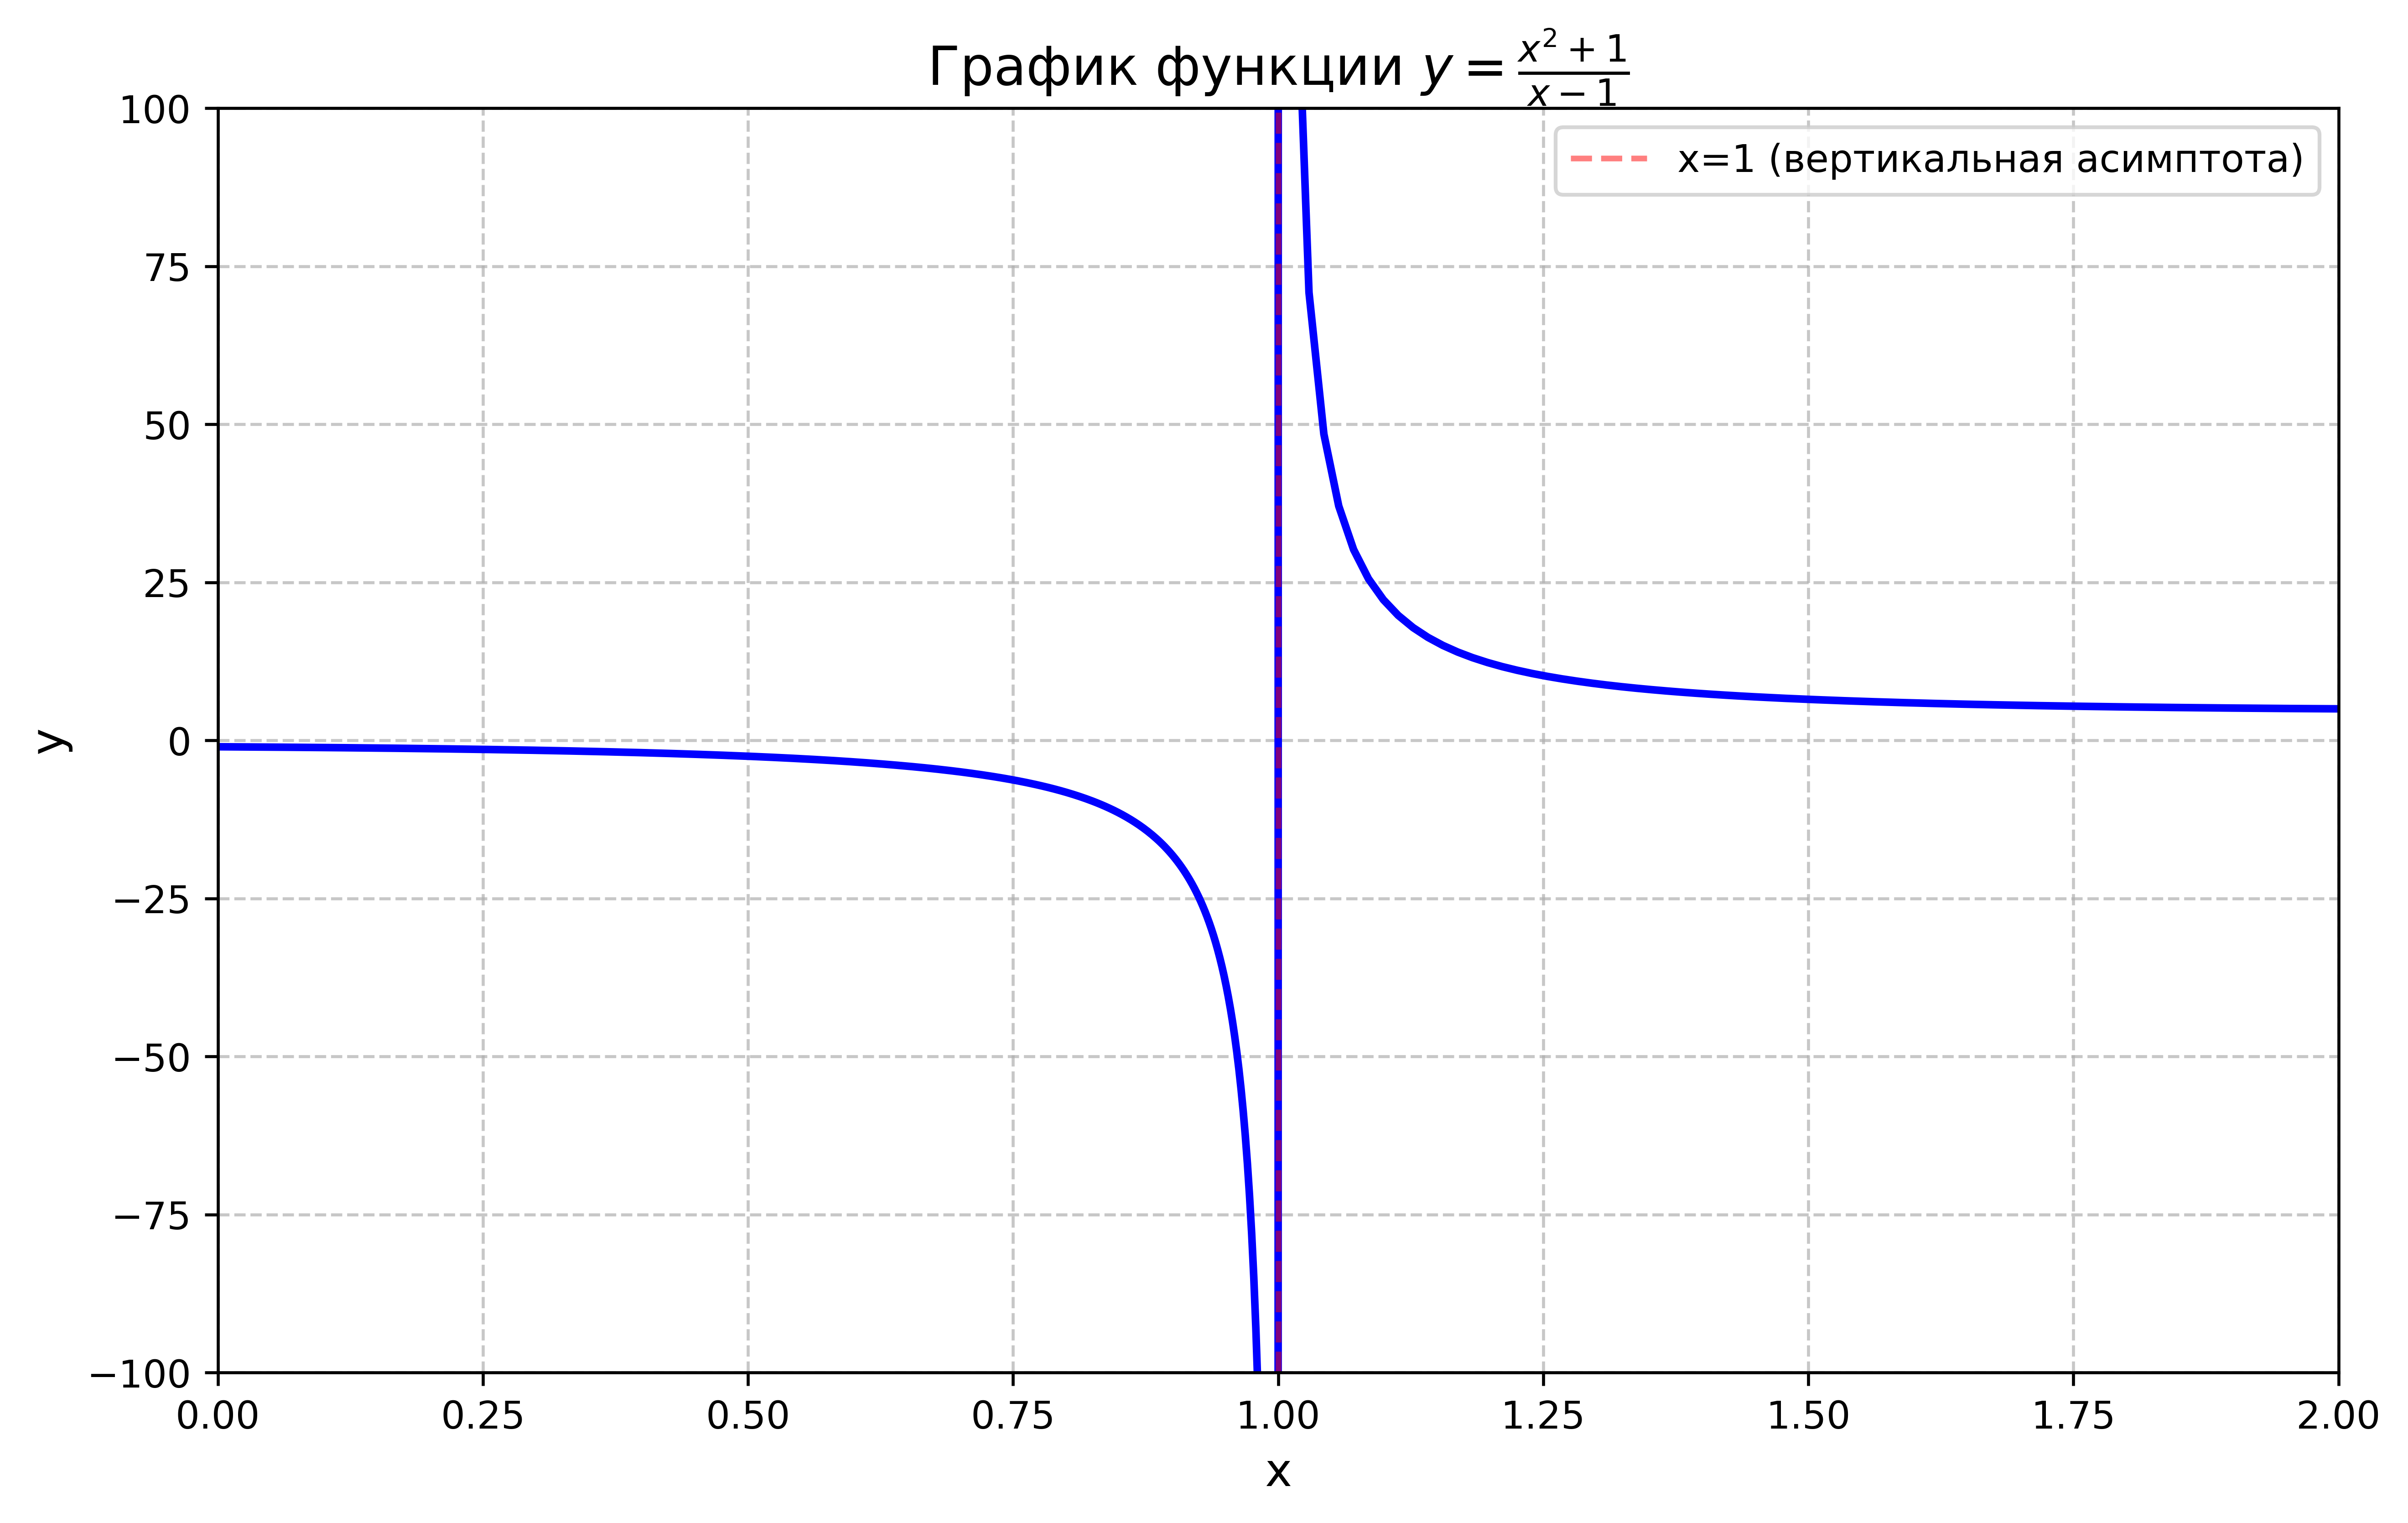
\includegraphics[width=0.8\textwidth]{../img/task1_graph.png}
    \caption{График функции \( f(x) = \frac{x^2 + 1}{x - 1} \)}
    \label{fig:graph}
\end{figure}

\emph{Решение задачи:}

\begin{figure}[H]
    \centering
    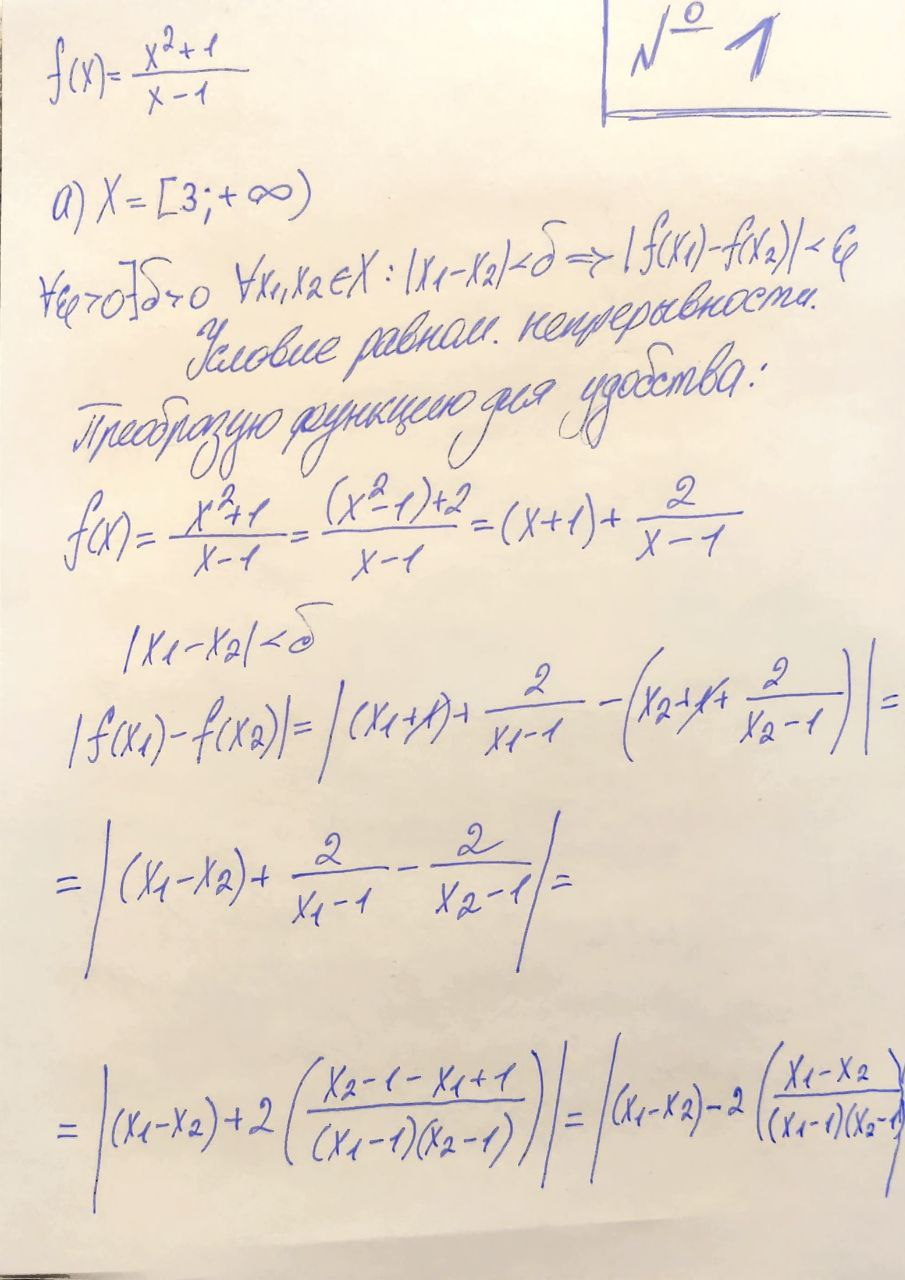
\includegraphics[width=0.8\linewidth]{../img/1_1.jpg}
    \caption{\emph{(a)}}
    \label{fig:part1}
\end{figure}

\begin{figure}[H]
    \centering
    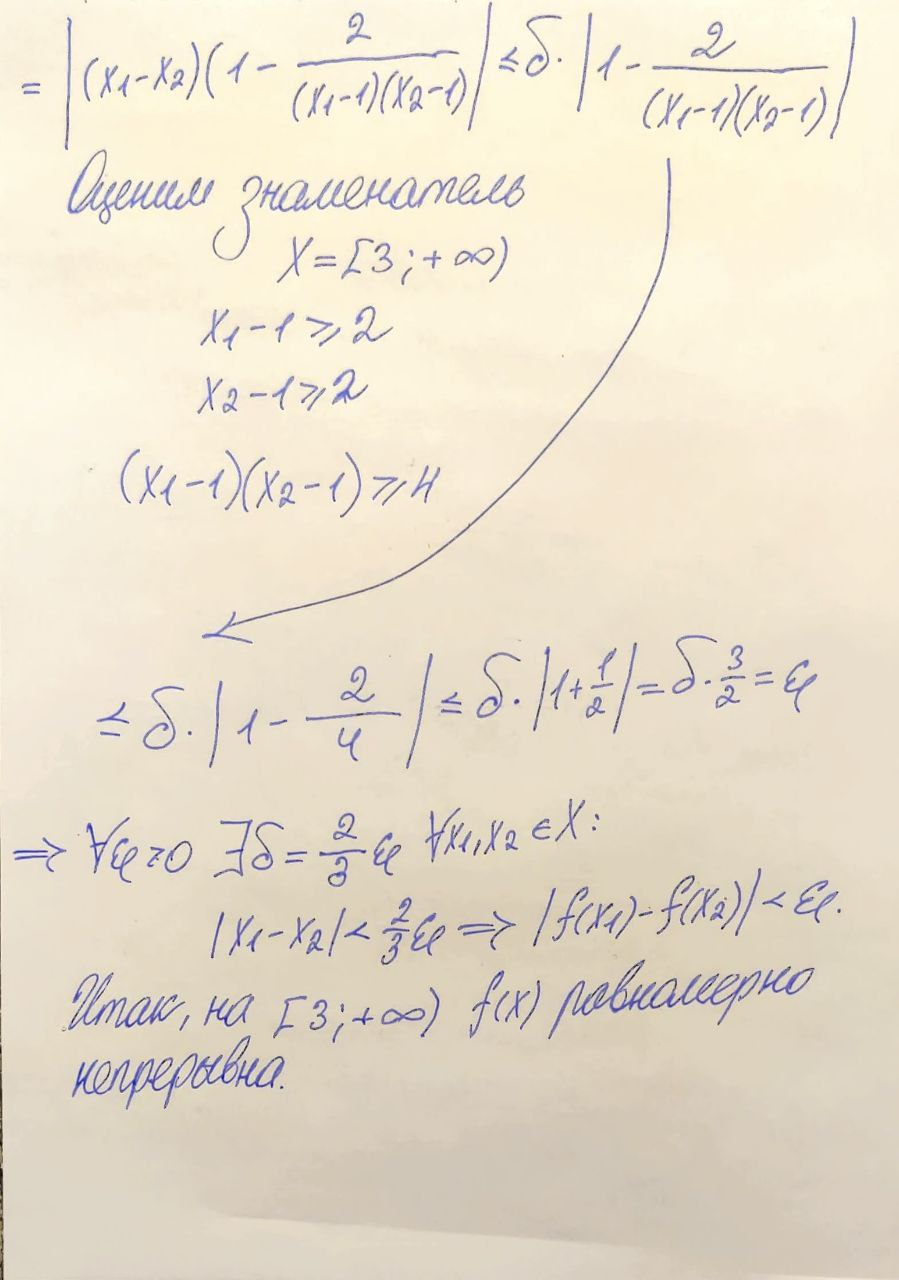
\includegraphics[width=0.8\linewidth]{../img/1_2.jpg}
    \caption{\emph{(a)}}
    \label{fig:part2}
\end{figure}

\begin{figure}[H]
    \centering
    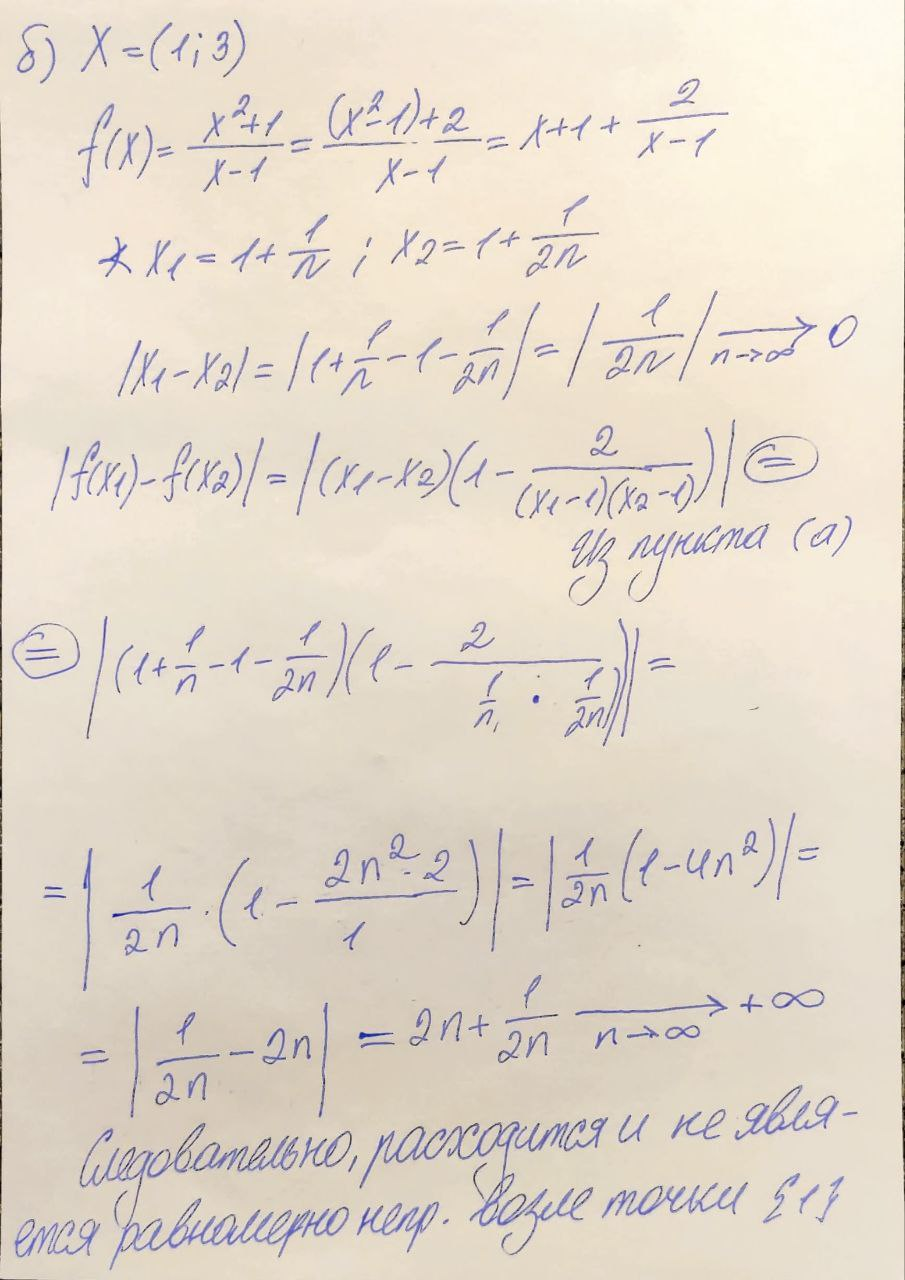
\includegraphics[width=0.8\linewidth]{../img/1_3.jpg}
    \caption{\emph{(b)}}
    \label{fig:part3}
\end{figure}

Итак, задача решена. Функция \( f(x) \) является равномерно непрерывной на промежутке \(X = [3,+\infty)\), и не является таковой на промежутке \( X = (1,3) \).

\end{document}